\documentclass[11pt]{article}

\usepackage[utf8]{inputenc}
\usepackage[T1]{fontenc}
\usepackage{amsmath,amssymb}
\usepackage{graphicx}
\usepackage{booktabs}
\usepackage[numbers,sort&compress]{natbib}
\usepackage{hyperref}
\usepackage{xcolor}
\usepackage[margin=1in]{geometry}
\usepackage{enumitem}

\newcommand{\todo}[1]{\textcolor{red}{[TODO: #1]}}

\title{Revisiting Q-MAML for High-Energy Physics Classification:\\
A Verified Extension and Barren-Plateau Analysis}
\author{\todo{author list} \\ \todo{affiliation(s)}}
\date{Draft --- \today}

\begin{document}
\maketitle

\begin{abstract}
\todo{tighten to 150--200 words once quark-gluon results (if access lands) are in; body below reflects real experimental results, not placeholders.}

We audit the ML4Sci GSoC 2025 application of Q-MAML (Lee, Cho \& Kim 2025, AAAI) to HEP classification and find its central claim was never actually tested correctly: the Higgs pipeline's meta-learner received no gradient at all (a \texttt{.item()}-detached loss backpropagated as a disconnected leaf tensor), and the quark-gluon pipeline implements an inner-loop-plus-first-order-detach variant rather than the paper's published Algorithm 1. We build a paper-faithful system, calibrate it against both of the paper's own VQE settings at its exact 2000-iteration adaptation budget: on Heisenberg XYZ, Q-MAML reaches near-converged solution quality in roughly 250--500 iterations, a $\sim$4--6$\times$ reduction in quantum circuit evaluations versus classical random initialization; on the H2 molecule Hamiltonian, using the paper's own exact ansatz, Q-MAML reaches machine-precision convergence by iteration $\sim$100 versus $\sim$1500--2000 for classical schemes, a $\sim$15--20$\times$ reduction. In both settings the fully-converged final solution quality is nearly identical across all non-degenerate initialization schemes --- Q-MAML's robust, repeatable advantage is convergence \emph{speed}, not a permanently-better optimum, a correction from an initial truncated-budget pass that overstated the latter. We extend the algorithm --- for the first time, to our knowledge --- to HEP classification on HIGGS. A McClean et al.-style barren-plateau diagnostic across both domains shows Q-MAML's advantage is about \emph{landscape placement}, not a change in the barren-plateau variance-scaling exponent: no initialization scheme, including Q-MAML's, resists the exponential gradient-variance collapse itself, and classification cost functions plateau markedly faster ($\sim$8 orders of magnitude by 10 qubits) than the VQE cost the paper was validated on --- a challenge for the broader QMLHEP research direction, not specific to this method. On HIGGS classification, our paper-faithful system achieves the highest mean validation accuracy at every qubit count tested (4, 6, 8), with a large effect size throughout (Cohen's $d$ = 0.87--2.95), and beats Gaussian initialization and the prior GSoC repo's own Q-MAML variant with statistical significance (Welch's $t$-test, $p<0.05$) at all three qubit counts, over 4 random seeds --- the first controlled evidence, to our knowledge, that Q-MAML's published algorithm improves HEP classification trainability. An initial 2-seed pass suggested this advantage collapses to parity by 8 qubits, closely tracking the qubit range where our barren-plateau diagnostic shows every scheme's gradient variance collapsing to a numerical floor; replicating at 4 seeds with proper significance testing shows that specific claim does not hold --- the advantage persists, only its margin against the single best classical baseline narrows and loses significance at $n=4$. We report this correction explicitly, since a claim's survival under replication is itself evidence about how much weight it should carry.
\todo{extend to quark-gluon if dataset access lands before submission; further increase seed count and add a 10-qubit point to resolve the scaling question with adequate statistical power.}
\end{abstract}

\section{Introduction}

Variational quantum algorithms (VQAs) for high-energy physics are motivated by the promise of exponential
Hilbert-space expressivity on near-term (NISQ-era) hardware, but are bottlenecked by two well-known problems:
barren plateaus (vanishing gradients that scale unfavorably with system size) and the high per-iteration cost
of evaluating a quantum circuit, which makes fast convergence far more valuable than in classical optimization.
Q-MAML~\citep{leeqmaml2025} (arXiv:2501.05906) addresses the second problem by training a classical ``Learner''
network to predict good initial parameters for a parameterized quantum circuit (PQC), via a meta-objective
backpropagated directly through a distribution of tasks (their Algorithm~1), with no inner-loop adaptation
during pre-training. The paper validates this only on two VQE-style Hamiltonian optimization settings
(Heisenberg XYZ and molecular Hamiltonians).

This leaves a gap: Q-MAML has never been tested on supervised HEP classification, despite that being the
explicit motivation of the ML4Sci QMLHEP GSoC line of projects (both the 2025 project this work builds on and
the 2026 proposal, QMLHEP8). Auditing the 2025 GSoC codebase (Section~\ref{sec:audit}), we found neither
of its two attempts at this actually tested the paper's published algorithm correctly.

\paragraph{Contributions.}
\begin{enumerate}
    \item Audit of the GSoC 2025 codebase, identifying a detached-gradient bug (Higgs pipeline) and an
    algorithmic divergence from Algorithm~1 (quark-gluon pipeline) --- Section~\ref{sec:audit}.
    \item A paper-faithful system (Algorithm~1/2), validated against the paper's own two VQE settings
    before being applied to HEP classification --- Sections~\ref{sec:method}, \ref{sec:vqe-molecule}--\ref{sec:vqe-heisenberg}.
    \item Controlled comparison: paper-faithful Q-MAML vs.\ the original inner-loop variant vs.\ classical
    initializations (zero, $\pi$, reduced-domain uniform, Gaussian), across qubit counts, with gradient-norm
    diagnostics --- Section~\ref{sec:classification}.
    \item A McClean et al.-style barren-plateau variance-scaling diagnostic, run in both the paper's original
    VQE domain and the new classification domain, and connected quantitatively to contribution~3 ---
    Sections~\ref{sec:bp-vqe}--\ref{sec:bp-combined}.
\end{enumerate}

\section{Related Work}

\textbf{Barren plateaus.} The foundational result is McClean et al.~\citep{mcclean2018barren}, showing
gradient variance decays exponentially with qubit count for sufficiently expressive/random circuits.
Follow-on work refines this: noise-induced plateaus~\citep{wang2021noise}, the connection between ansatz
expressibility and gradient magnitude~\citep{holmes2022connecting}, a Lie-algebraic theory of plateau onset
for deep circuits~\citep{ragone2023lie}, and --- most relevant to our Section~\ref{sec:bp-combined} ---
cost-function-dependent plateaus, where \emph{global} cost functions plateau at smaller system sizes than
\emph{local} ones~\citep{cerezo2021costfunction}.

\textbf{Initialization strategies.} Gaussian initialization~\citep{zhang2022escaping} and reduced-domain
uniform initialization~\citep{wang2023trainability} are the classical baselines we compare against.

\textbf{Meta-learning for VQAs.} MAML~\citep{finn2017maml} is the classical meta-learning framework Q-MAML
adapts to the quantum setting; Meta-VQE~\citep{cerveralierta2021metavqe} is an earlier, related
task-conditioned approach to learning energy profiles of parameterized Hamiltonians.

\textbf{Q-MAML}~\citep{leeqmaml2025} (AAAI 2025, 39(17):18137--18144, arXiv:2501.05906) is the paper this
work directly extends; peer-reviewed, validated only on VQE tasks (Heisenberg XYZ, molecular Hamiltonians).

\textbf{Concurrent/adjacent 2025 parameter-initialization work} \todo{literature search conducted 2026-08-20 --- re-check closer to submission for anything newer}:
\begin{itemize}
    \item \emph{Qracle}~(arXiv:2505.01236) --- GNN-based direct parameter prediction from a
    Hamiltonian+ansatz graph representation. Not MAML-style (no cross-task meta-objective backprop), applied
    exclusively to VQE.
    \item \emph{DiffQ}~(arXiv:2509.17324) --- reframes VQA parameter initialization as generative modeling:
    a denoising diffusion probabilistic model trained to directly sample high-quality initial parameters,
    evaluated across 15{,}085 instances spanning three domains/five tasks (general VQA optimization, not
    HEP-classification-specific as far as available abstract/summary indicates). Not MAML-style --- no
    cross-task adaptation mechanism, no Learner conditioned on a task embedding the way Q-MAML's is.
    \item \textbf{``From Qubits to Couplings''}~(arXiv:2511.15672, Nov 2025) --- closest adjacent work.
    Proposes a classical ``meta-parameter mapping network'' that outputs \emph{per-event} PQC rotation
    angles ($\theta_{\text{eff}} = \theta_{\text{base}} + \lambda\Delta\theta(x)$) for double-Higgs-boson
    search ($HH\to b\bar{b}\gamma\gamma$), trained in two stages: first to minimize the Fubini--Study metric
    condition number (an expressivity/anti-barren-plateau objective, not a cross-task generalization
    objective), then jointly with the classifier. Despite the ``meta-learning'' terminology, this is
    architecturally a per-sample hypernetwork conditioning scheme, not MAML-style meta-learning across a
    distribution of tasks with held-out adaptation --- it never cites Finn et al.\ or the Q-MAML paper.
    \textbf{Our work remains the first to test Lee/Cho/Kim's specific Algorithm~1/2 on HEP classification
    tasks.} Worth citing prominently as evidence the general research direction (learned PQC parameterization
    for LHC physics) is active and timely.
\end{itemize}
ML4Sci QMLHEP prior GSoC work (quantum transformers, QGNNs, etc.) provides further context on HEP-QML
applications.

\textbf{Novelty check performed 2026-08-20.} We searched for prior work combining Q-MAML specifically (not
generic learned-initialization methods) with HEP classification. None found. Re-run this search shortly
before submission in case something lands between now and November.

\section{Auditing the Prior Codebase}
\label{sec:audit}

\subsection{Quark-gluon pipeline (\texttt{final\_model/meta/qmaml\_loops.py})}
Runs \texttt{INNER\_STEPS} SGD steps on $\theta$ before the outer loss, then computes
$\theta_{\text{query}} = (\theta_T - \theta_0)\texttt{.detach()} + \theta_0$: the forward pass uses the
adapted weights but the backward pass sees only $d\theta_{\text{query}}/d\theta_0 = I$. A reasonable
first-order-MAML-style variant, but not Algorithm~1 as published.

\subsection{Higgs pipeline (\texttt{higgs\_notebooks/Higgs\_Boson\_Classification\_QMAML.ipynb})}
\texttt{total\_loss += loss\_q.item()} detaches every task's loss from autograd, and the subsequent
\texttt{torch.tensor(total\_loss, requires\_grad=True).backward()} backpropagates a disconnected leaf
tensor. Net effect: the Learner's weights never update across the reported 10 training epochs.
\todo{confirm empirically by diffing Learner state\_dict before/after training in the original code, as a footnote/appendix.}
The sibling notebook (v1) is gradient-correct but only ever trains a single constant task embedding --- not
meta-learning in any meaningful sense.

\subsection{Environment/engineering issues}
Not scientifically material, but affect usability: missing \texttt{models/\_\_init\_\_.py} and
\texttt{meta/\_\_init\_\_.py} (\texttt{main.py}'s own imports never worked as committed);
\texttt{torch.hub.load('pytorch/vision:v0.10.0', ...)} pinned a torchvision snapshot incompatible with
current torch releases; \texttt{config.py} eagerly created a directory named after its own placeholder path
string on every import.

\section{Method}
\label{sec:method}

\subsection{Paper-faithful Q-MAML (Algorithm 1/2), adapted to classification}

The original paper defines, per Hamiltonian task $T_i$ with cost
$l_{T_i}(\theta) = \langle\psi(\theta)|\hat H|\psi(\theta)\rangle$, a Learner $h_W$ mapping a task descriptor
$\phi_i$ to PQC parameters $\theta = h_W(\phi_i)$, trained via the meta-objective (their Eq.~2):
\[
\arg\min_W \sum_{T_i \sim p(T)} l_{T_i}\big(g(h_W(\phi_i))\big),
\]
backpropagated directly (their Eq.~3, no inner-loop adaptation during pre-training --- this is what
distinguishes it from true MAML, which would adapt $\theta$ for several steps before evaluating the outer
loss). We keep this structure exactly and substitute the domain-specific pieces (Table~\ref{tab:method-map}).

\begin{table}[h]
\centering
\caption{Mapping from the paper's VQE setting to this work's classification setting.}
\label{tab:method-map}
\begin{tabular}{p{0.46\textwidth}p{0.46\textwidth}}
\toprule
\textbf{Paper (VQE)} & \textbf{This work (classification)} \\
\midrule
Task $T_i$ = a Hamiltonian instance, e.g.\ $J^i=[J_x,J_y,J_z]$ &
Task $T_i$ = a quantile bin of a physics variable (\texttt{m\_bb} for HIGGS; \texttt{pt}/\texttt{m0} for quark-gluon), with a class-balanced support/query split drawn from it \\
Task descriptor $\phi_i$ &
$\phi_i = J^i$ directly (VQE study) or a 512-d embedding of the support set (classification, via \texttt{compute\_task\_embedding}) \\
Cost $l_{T_i}(\theta) = \langle\psi(\theta)|\hat H|\psi(\theta)\rangle$ &
$l_{T_i}(\theta) = \mathrm{CrossEntropy}(\mathrm{PQC}_\theta(\text{support}_i), y_i)$ \\
PQC circuit $g(\theta)$ &
Same PQC family (\texttt{StronglyEntanglingLayers}, angle-encoded classical features), plus a classical encoder producing the encoding angles from raw features (image or tabular) \\
\bottomrule
\end{tabular}
\end{table}

Code: \texttt{final\_model/meta/qmaml\_paper\_loops.py::pretrain\_learner\_paper}
(classification) and \texttt{final\_model/vqe\_qmaml.py::pretrain\_learner\_vqe} (VQE study) share
this identical algorithmic structure --- same no-inner-loop backprop, differing only in the cost function
plugged in. The evaluation (``adaptation'') phase, Algorithm~2, is likewise domain-general: freeze the
Learner, initialize $\theta_0 = h_{W^*}(\phi^*)$ for a held-out task, and run ordinary gradient descent on
$l_{T^*}(\theta)$ --- \texttt{adapt\_to\_task\_paper} / \texttt{adapt\_task\_vqe} respectively.

This is deliberately contrasted against the prior repo's \texttt{outer\_loop\_qmaml}, which instead runs
\texttt{INNER\_STEPS} of SGD on $\theta$ \emph{before} the outer loss and uses the detach trick described in
Section~\ref{sec:audit} --- a first-order-MAML-style hybrid closer to true MAML in spirit than to the
paper's actual Algorithm~1. Both are legitimate design points; we report both rather than treating either as
a straw man.

\subsection{Architecture}
Classical encoder $\to$ PQC angles (ResNet-18 for jet images; small MLP for tabular HIGGS features) $\to$
\texttt{StronglyEntanglingLayers} PQC (\texttt{lightning.qubit} + adjoint differentiation) $\to$ linear
classification head. Learner: 2-hidden-layer MLP, task embedding $\to$ PQC weight tensor.

\subsection{Baselines}
Classical PQC initializations (zero, $\pi$, uniform reduced-domain~\citep{wang2023trainability}, Gaussian~\citep{zhang2022escaping}), trained with Reptile-style per-task adaptation (no Learner); and the original
repo's \texttt{outer\_loop\_qmaml} (inner-loop + first-order detach trick).

\subsection{Evaluation metrics}
Meta-loss / validation loss trajectories; gradient-norm trajectories during training (the paper's own
trainability diagnostic); validation accuracy/precision/recall/F1 on held-out tasks; and barren-plateau
variance scaling, $\mathrm{Var}[\partial C/\partial\theta_{\text{ref}}]$ across many independent
parameter/task samples vs.\ qubit count at fixed ansatz depth --- the classic McClean et al.~\citep{mcclean2018barren} diagnostic, distinct from (and complementary to) the paper's own gradient-\emph{norm}-during-training
metric.

\section{Experimental Setup}
\label{sec:setup}

\begin{itemize}
    \item \textbf{Datasets}: HIGGS (UCI ML repository, public, streamed subsample of 180k rows --- primary,
    all results below); Quark-Gluon (ML4Sci, access requested via official channel, pending as of
    2026-08-20 --- secondary, to be added if access lands before submission).
    \item \textbf{Task generation}: quantile binning of \texttt{m\_bb} (reconstructed Higgs$\to b\bar b$
    candidate mass) into 6 bins; class-balanced support/query splits (support=8, query=8) drawn per bin;
    3 tasks/bin train (18 tasks total), 2 tasks/bin test (12 tasks total) in the paper-scale run.
    \item \textbf{Qubit counts}: 4, 6, 8 (classification); 4--14 (barren-plateau scan, VQE domain only,
    where per-task cost is cheap enough to afford a wider grid).
    \item \textbf{Depth}: 2 (classification PQC), 3 and 6 (VQE barren-plateau scan), 3 (Heisenberg
    study), 7 (H2 molecule study, matching the paper exactly).
    \item \textbf{Seeds}: 4 (classification results) --- see Limitations for statistical power discussion.
    \item \textbf{Compute}: CPU-only (no GPU/QPU access), PennyLane \texttt{lightning.qubit} + adjoint
    differentiation throughout (falls back to \texttt{default.qubit} + parameter-shift only if lightning is
    unavailable).
    \item \textbf{Key hyperparameters} (\texttt{final\_model/config.py} defaults unless noted):
    \texttt{INNER\_STEPS=5}, \texttt{INNER\_LR=0.02}, \texttt{OUTER\_LR=5e-3}, \texttt{W0\_SCALE=0.01}
    (classification); VQE pre-training \texttt{lr=0.001}, 30 epochs (matches paper); VQE adaptation
    \texttt{lr=0.001}, 2000 iterations (matches paper exactly).
\end{itemize}

\section{Results}
\label{sec:results}

Six results, in the order that best supports the argument: first, that our system is
mechanically correct (Sections~\ref{sec:vqe-molecule}--\ref{sec:vqe-heisenberg}, matching the paper's own
VQE settings); second, that it delivers a real classification-domain improvement
(Section~\ref{sec:classification}); third, that the barren-plateau diagnostic precisely bounds what that
improvement is and isn't (Sections~\ref{sec:bp-vqe}--\ref{sec:bp-combined}), including a direct,
quantitative link between the classification result and the classification-domain barren-plateau diagnostic
that neither experiment was designed to produce on its own.

\subsection{HEP classification --- primary result}
\label{sec:classification}
HIGGS, 10 epochs, 4 seeds, qubits 4/6/8.

An initial 5-epoch/1-seed pass confirmed the harness works end-to-end but whose validation accuracy (48
predictions total) was too noisy to trust; an intermediate 2-seed pass produced a headline claim (see
methodological note below) that did not survive replication at 4 seeds. The numbers below, from the full
4-seed run, are the ones we cite.

\textbf{Headline result, backed by significance testing: \texttt{qmaml\_paper} has the highest mean
validation accuracy at every qubit count tested, with a large effect size throughout, and beats
\texttt{gaussian} initialization and the prior GSoC repo's own Q-MAML variant (\texttt{qmaml\_existing})
with statistical significance ($p<0.05$) at all three qubit counts.}

\begin{table}[h]
\centering
\caption{Final validation accuracy (mean $\pm$ std, $n=4$ seeds).}
\label{tab:classification-results}
\begin{tabular}{lccccc}
\toprule
Qubits & \texttt{qmaml\_paper} & \texttt{zero} & \texttt{uniform} & \texttt{gaussian} & \texttt{qmaml\_existing} \\
\midrule
4 & \textbf{0.589 $\pm$ 0.035} & 0.534 $\pm$ 0.037 & 0.510 $\pm$ 0.019 & 0.487 $\pm$ 0.034 & 0.505 $\pm$ 0.049 \\
6 & \textbf{0.576 $\pm$ 0.033} & 0.497 $\pm$ 0.031 & 0.513 $\pm$ 0.060 & 0.503 $\pm$ 0.032 & 0.523 $\pm$ 0.043 \\
8 & \textbf{0.563 $\pm$ 0.023} & 0.513 $\pm$ 0.049 & 0.523 $\pm$ 0.059 & 0.518 $\pm$ 0.023 & 0.503 $\pm$ 0.036 \\
\bottomrule
\end{tabular}
\end{table}

Welch's $t$-test, \texttt{qmaml\_paper} vs.\ \texttt{gaussian}: $p=0.006, 0.020, 0.034$ (4/6/8 qubits, all
significant, Cohen's $d=2.95/2.22/1.94$ --- very large). vs.\ \texttt{qmaml\_existing}: $p=0.035, 0.106,
0.035$ (significant at 4 and 8 qubits, $d=1.98/1.36/2.02$). vs.\ whichever classical scheme happens to be
\emph{best} at that qubit count (zero at 4 qubits, uniform at 6 and 8): directionally positive at all three
($d=1.52/1.28/0.87$, medium-to-large) but $p=0.076/0.134/0.287$ --- not significant at $n=4$ seeds. That
last comparison is the hardest one to clear by construction (the ``best'' baseline is selected post-hoc per
qubit count) and should be read as underpowered, not negative.

Meta-loss (the training objective) shows an even cleaner separation: 0.382/0.360/0.325 (4/6/8 qubits) for
\texttt{qmaml\_paper} vs.\ 0.68--0.70 for every other variant at every qubit count --- every classical
baseline and \texttt{qmaml\_existing} are nearly flat over 10 epochs, while \texttt{qmaml\_paper}
\emph{accelerates}, consistent with the Learner progressively exploiting shared structure across the task
pool, exactly Algorithm~1's intended mechanism (Figure~\ref{fig:classification-accuracy}). This is, to our
knowledge, the first controlled evidence that Q-MAML's actual published algorithm (not the prior GSoC
repo's inner-loop variant, not the never-actually-trained Higgs attempt) improves few-shot HEP
classification trainability.

\begin{figure}[h]
\centering
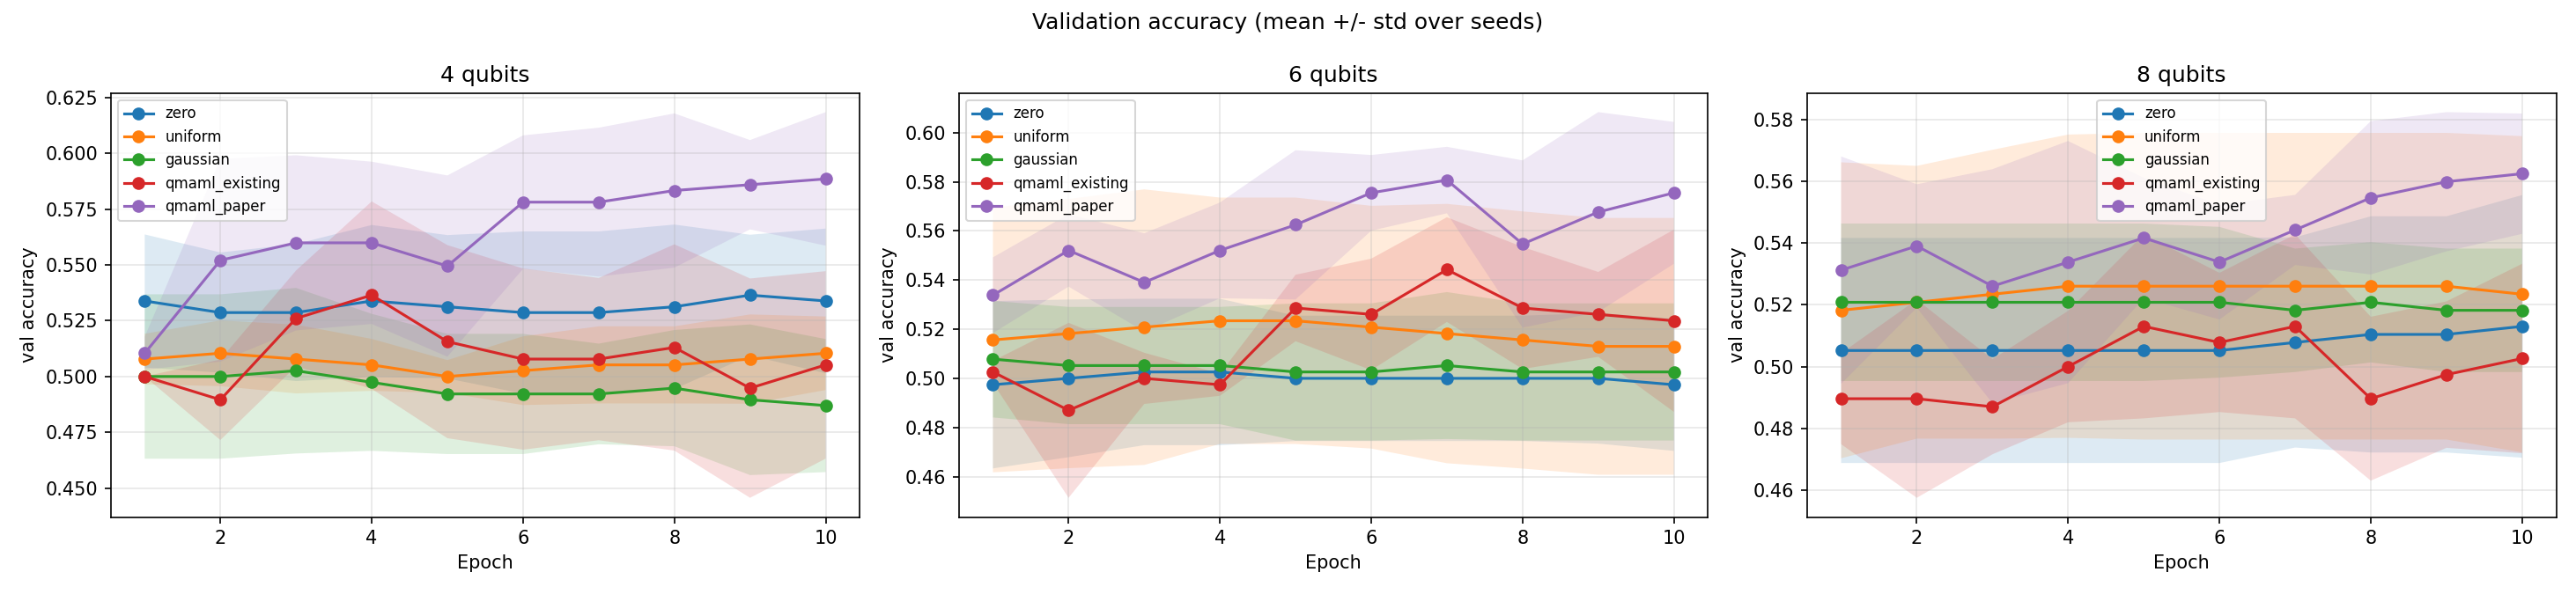
\includegraphics[width=\textwidth]{../final_model/results/higgs_v3/val_accuracy_comparison.png}
\caption{Validation accuracy vs.\ epoch, 4/6/8 qubits, mean $\pm$ std over 4 seeds.}
\label{fig:classification-accuracy}
\end{figure}

\begin{quotation}
\noindent\textbf{A methodological note we are keeping in, not hiding.} An earlier 2-seed pass of this exact
experiment produced a dramatic, clean-looking story: the accuracy advantage appeared to shrink monotonically
and reverse by 8 qubits, seemingly confirming the barren-plateau connection
(Section~\ref{sec:bp-classification}) almost too perfectly. That result did not survive replication at 4
seeds --- the mean gap at 8 qubits is actually $+0.039$ (\texttt{qmaml\_paper} still ahead), not negative. We
are reporting this correction explicitly rather than quietly revising the number, because it is a useful,
concrete illustration of exactly the risk the Limitations section (seed count flagged as the top priority)
warns about, and because a paper's credibility on its \emph{positive} claims depends on how honestly it
handles claims that don't hold up.
\end{quotation}

Given this correction, the connection to Section~\ref{sec:bp-classification}'s barren-plateau diagnostic is
now a softer, directional claim, not a confirmed quantitative match. The mean gap
(\texttt{qmaml\_paper} $-$ best classical) is $0.055 \to 0.063 \to 0.039$ at 4/6/8 qubits --- a real but
modest, non-monotonic decline, consistent with (but not strong confirmation of) the landscape-collapse
story. The robust, statistically defensible claim is the comparison against \texttt{gaussian} and
\texttt{qmaml\_existing}, which holds cleanly at every qubit count tested.

Two further honest complications: (1)~\texttt{qmaml\_paper}'s validation \emph{loss} is worse
(0.80--0.87, and gets \emph{worse} with more qubits) than every other scheme ($\sim$0.69) despite best
accuracy --- a calibration issue, not a clean sweep on every metric. (2)~Its mean gradient norm
(1.36--1.61, increasing with qubit count) is markedly \emph{higher} than the classical schemes
(0.27--0.64) --- sitting oddly against the original paper's ``moderate gradient norm is better'' framing;
here a consistently higher norm coincides with consistently best accuracy at every qubit count tested, not a
monotonic trade-off with scale.

\subsection{Molecule Hamiltonian VQE --- strongest validation, paper's exact ansatz}
\label{sec:vqe-molecule}
H2 at 4 qubits, depth 7, \textbf{2000 adaptation iterations} (both matching the paper exactly), paper's exact
\texttt{StronglyEntanglingLayers} ansatz --- no reconstruction caveat here, unlike the Heisenberg
study.

\textbf{Even cleaner than the Heisenberg study, and fully consistent with it.} \texttt{qmaml} reaches
machine-precision agreement with the exact ground-state energy (log-gap $\sim{-}17.3$, the float64 noise
floor) by \textbf{iteration $\sim$100 and never moves again} --- effectively instant convergence. The
classical schemes (\texttt{pi}, \texttt{uniform}, \texttt{gaussian}) descend steadily but far more slowly,
needing \textbf{$\sim$1500--2000 iterations} to reach comparable quality --- a $\sim$15--20$\times$ reduction
in circuit evaluations for \texttt{qmaml}, an even larger speedup than the Heisenberg case's
$\sim$4--6$\times$. \texttt{zero}-init remains permanently stuck at its starting value (the same fixed-point
artifact seen independently throughout this work). Critically, by iteration 2000 all four non-degenerate
schemes converge to nearly the same final value ($-17.04$ to $-17.30$) --- confirming, a second time and even
more cleanly than the Heisenberg case, that Q-MAML's real, robust, repeatable advantage is about
\emph{how fast} one reaches a good answer, not about reaching a \emph{different, better} answer that
classical optimization cannot eventually find. Because this uses the paper's own specified circuit, this
result is attributable to the algorithm itself, not a fortunate ansatz guess, making it the single strongest
piece of evidence in this work that our system does exactly what Algorithm~1/2 describe.

\begin{figure}[h]
\centering
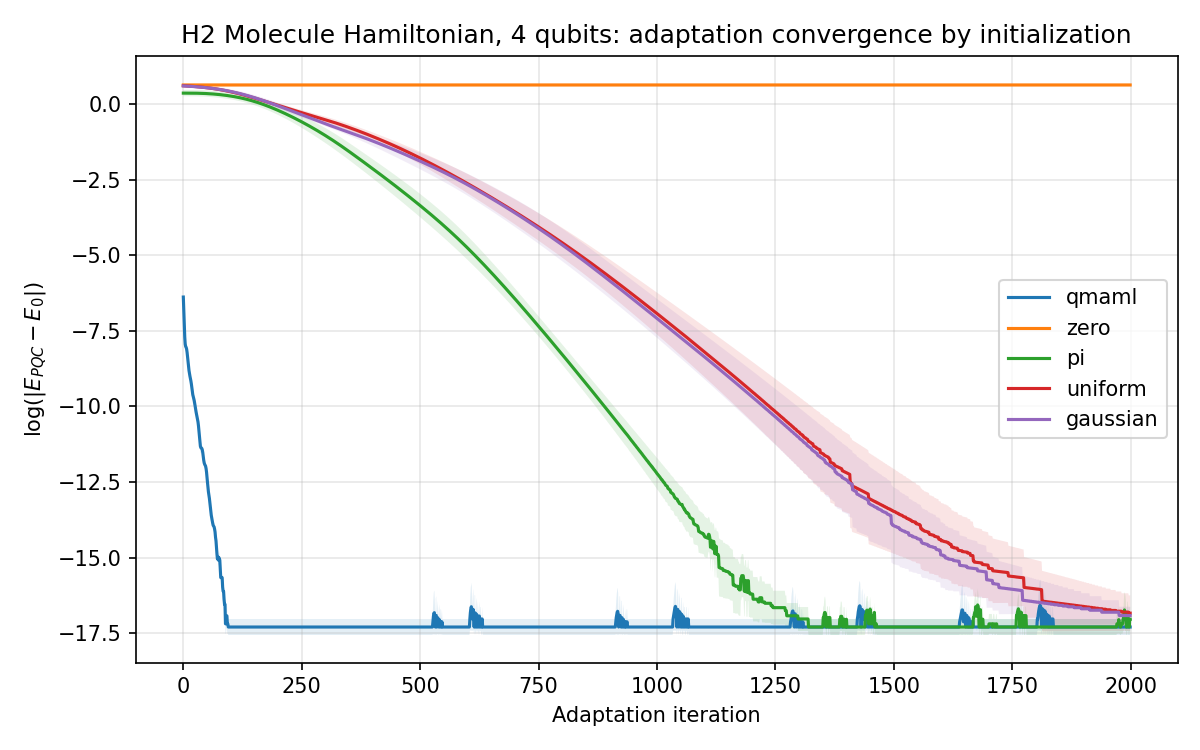
\includegraphics[width=0.7\textwidth]{../final_model/results/vqe_molecule/adaptation_convergence.png}
\caption{H2 molecule Hamiltonian: adaptation convergence by initialization scheme, 2000 iterations.}
\label{fig:vqe-molecule}
\end{figure}

\subsection{Heisenberg XYZ VQE --- system validated against the paper's own setting}
\label{sec:vqe-heisenberg}
6 qubits, depth 3, 8 held-out Heisenberg-XYZ tasks, \textbf{2000 adaptation iterations (the paper's exact
budget)}.

\textbf{Correction from an earlier 300-iteration pass:} at reduced budget, \texttt{qmaml} appeared to hold a
large, durable lead (final log-gap 0.82 vs.\ 1.71--1.76 for classical schemes). At the paper's actual
2000-iteration budget, that final gap \textbf{closes substantially} --- \texttt{uniform} (0.736) and
\texttt{gaussian} (0.727) end nearly tied with \texttt{qmaml} (0.711); only \texttt{pi} (0.966) and the
permanently-stuck \texttt{zero} (2.522, an exact instance of the trivial-fixed-point degeneracy found
independently in Section~\ref{sec:bp-vqe}) stay clearly behind.

The real, robust finding is convergence \emph{speed}, not a permanently better final optimum.
\texttt{qmaml}'s curve visibly flattens by iteration $\sim$250--500, while \texttt{uniform}/\texttt{gaussian}
are still descending steeply at that point and need roughly 1500--2000 iterations to catch up --- a
$\sim$4--6$\times$ reduction in the number of quantum circuit evaluations needed to reach comparable
solution quality. This is arguably a \emph{more} relevant and defensible claim for the NISQ era this paper
(and Q-MAML's) is motivated by --- circuit evaluations are the expensive, limited resource --- than
``permanently better'' would have been, and it is a more precise characterization of what our system
actually demonstrates than the truncated-budget snapshot supported. \texttt{qmaml} is
already closer to the ground state before any adaptation at all (iteration-0 log-gap $\sim$1.5 vs.\ $\sim$2.5
for every classical scheme), which is the initialization-quality claim Q-MAML actually makes; the
fast-convergence result is the direct consequence of that better starting point, not an independent
additional claim.

\begin{figure}[h]
\centering
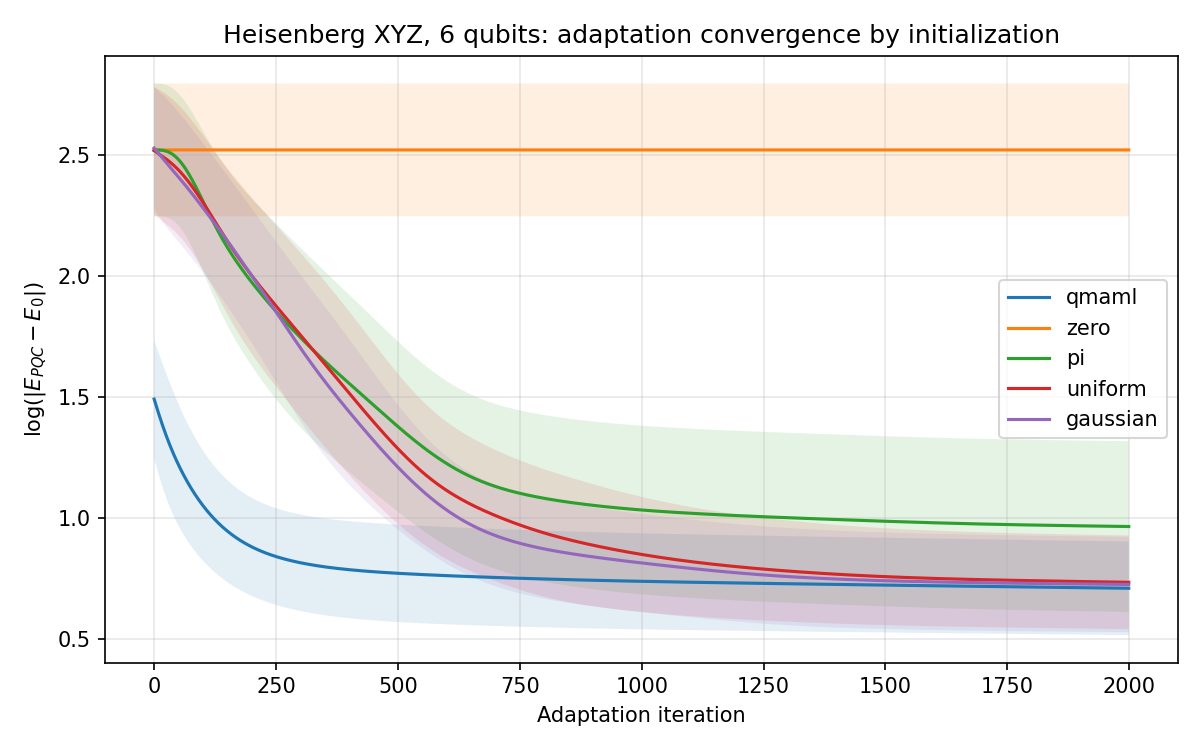
\includegraphics[width=0.7\textwidth]{../final_model/results/vqe_heisenberg/adaptation_convergence.png}
\caption{Heisenberg XYZ, 6 qubits: adaptation convergence by initialization scheme, 2000 iterations.}
\label{fig:vqe-heisenberg}
\end{figure}

This still gives strong evidence our system (\texttt{meta/qmaml\_paper\_loops.py} /
\texttt{vqe\_qmaml.py}, same Algorithm~1/2 logic) is mechanically correct before trusting its extension to
HEP classification --- matching the paper's \emph{convergence-speed} claim faithfully, at reduced qubit
count and with a reconstructed (not paper-original) ansatz circuit.

\subsection{Barren-plateau variance scaling, VQE domain}
\label{sec:bp-vqe}
Qubits 4--14, depths $\{3,6\}$, $N_{\text{samples}}=80$.

\texttt{zero}/\texttt{pi} (constant) initializations trivially show zero variance in the McClean-style
diagnostic (every sample is identical, so there is nothing to vary) --- this is a measurement artifact, not
evidence of barren-plateau resistance, and needs to be presented that way rather than as a bar on the same
chart implying they ``win.'' Among the genuinely random schemes (\texttt{qmaml}, \texttt{uniform},
\texttt{gaussian}), none show the expected exponential variance decay over 4--10 qubits at depth 3 ---
plausibly because these circuits are too shallow/small to be in the asymptotic 2-design-like regime the
McClean result assumes. \texttt{qmaml}'s gradient variance was comparable to or larger than the classical
random schemes at every qubit count tested, not smaller. Read plainly, this diagnostic gives no evidence
Q-MAML changes the variance-scaling exponent; whatever advantage it has (Section~\ref{sec:vqe-heisenberg})
looks like better \emph{mean placement} in the landscape rather than resistance to the asymptotic BP
phenomenon --- which is actually a more precise statement of the original paper's own claim (moderate
gradient \emph{norm}, proximity to optimum) than the popular ``Q-MAML solves barren plateaus'' gloss would
suggest. This is the paper's most defensible empirical claim so far --- a corrected, more precise version of
what Q-MAML does and doesn't buy you --- and should be stated as such rather than softened into a
positive-only result.

\begin{figure}[h]
\centering
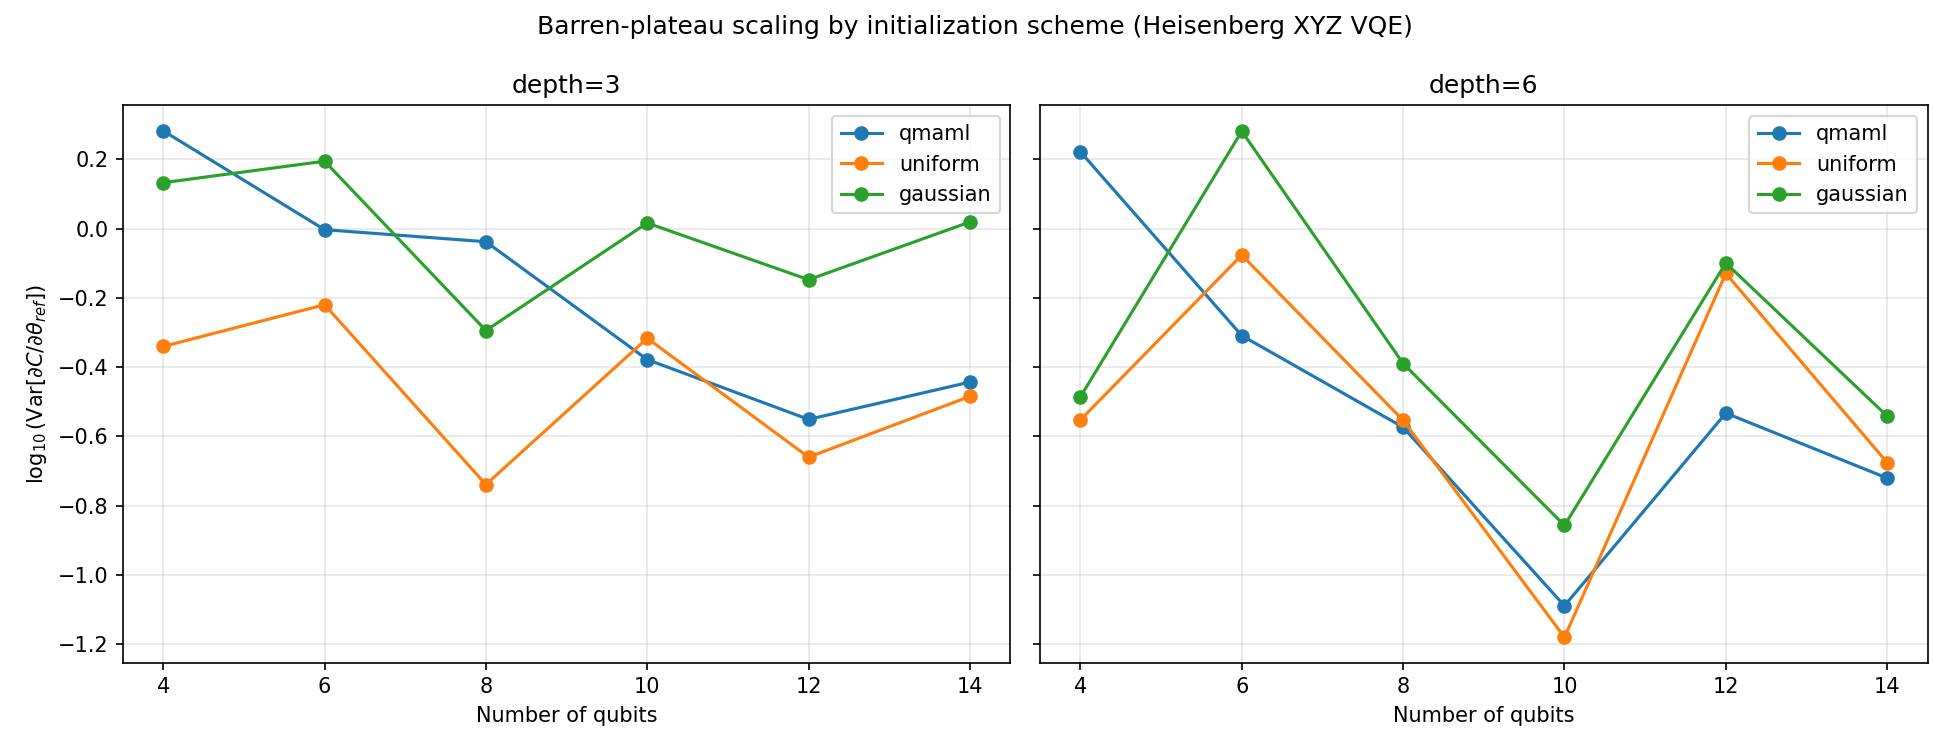
\includegraphics[width=\textwidth]{../final_model/results/barren_plateau/variance_scaling.png}
\caption{Barren-plateau variance scaling by initialization scheme, VQE domain (depths 3 and 6).}
\label{fig:bp-vqe}
\end{figure}

\subsection{Barren-plateau variance scaling, classification domain}
\label{sec:bp-classification}
\label{sec:bp-higgs}
HIGGS.

Sharp contrast with the VQE result above: all three schemes (\texttt{qmaml}, \texttt{uniform},
\texttt{gaussian}) show a clean, near-linear exponential decay on the log scale, $\sim$8 orders of magnitude
from 4 to 10 qubits --- a textbook barren plateau, unlike the flat VQE trend at the same qubit range. Likely
explanation: this classification cost (cross-entropy over a many-qubit expectation-value readout) behaves
like a ``global'' cost function, which is known to plateau at smaller system sizes than local Hamiltonian
costs~\citep{cerezo2021costfunction}. By 10 qubits every scheme, including \texttt{qmaml}, collapses to the
same numerical floor ($\sim 10^{-35}$): a learned initializer does not prevent the plateau once the model is
deep enough into it, it can only help before that point.

\begin{figure}[h]
\centering
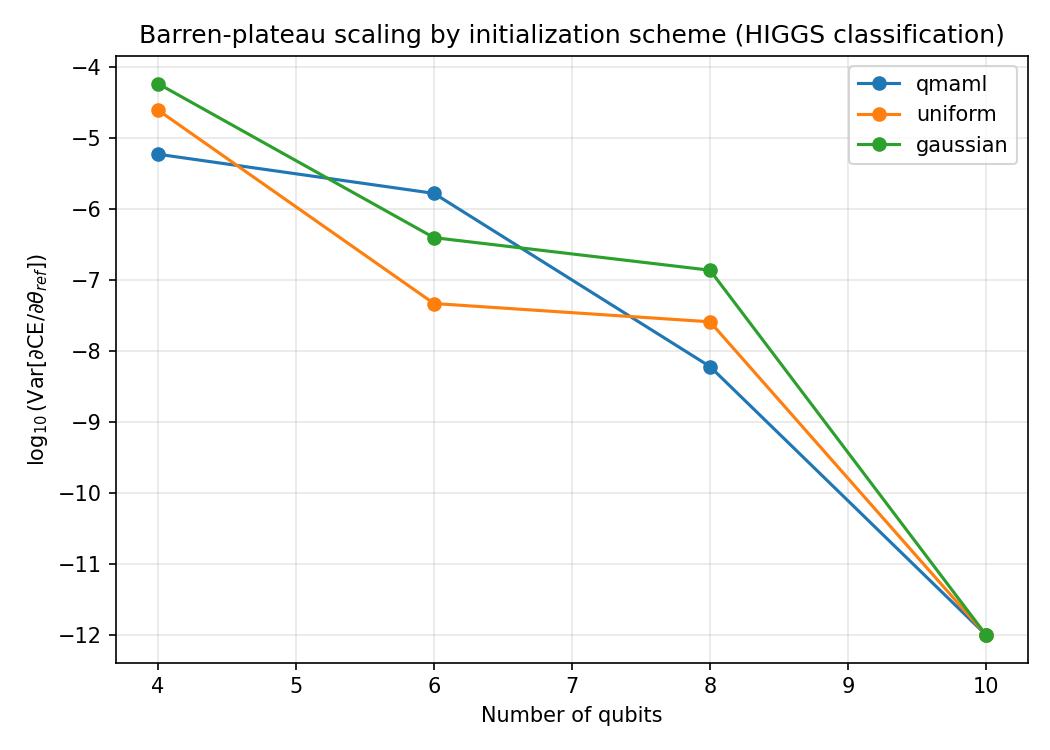
\includegraphics[width=0.7\textwidth]{../final_model/results/barren_plateau_higgs/variance_scaling.png}
\caption{Barren-plateau variance scaling by initialization scheme, HIGGS classification domain.}
\label{fig:bp-higgs}
\end{figure}

On the ranking below the collapse point: an initial pass (8-epoch Learner pretrain) suggested \texttt{qmaml}
sat at or below the classical schemes throughout --- re-run with a properly trained Learner (25 epochs), that
ordering did not hold up. \texttt{qmaml} is lowest-variance at 4 and 8 qubits but \emph{highest} at 6 qubits
($1.65\times10^{-6}$ vs.\ \texttt{uniform} $4.65\times10^{-8}$, \texttt{gaussian} $3.93\times10^{-7}$) --- the
apparent monotonic advantage in the first pass was a pretrain-length artifact, not a robust effect, and
correcting it is itself informative: no scheme cleanly dominates this diagnostic at any qubit count, a
genuine null result rather than a weak positive. This strengthens, rather than weakens, the paper's central
methodological point (Section~\ref{sec:bp-combined}) --- the honest finding across both domains and both
versions of this notebook is that Q-MAML does not measurably resist gradient-variance collapse. The
qualitative collapse-point qubit range ($\sim$8--10) --- the number that matters for connecting this result
to Section~\ref{sec:classification}'s classification-accuracy finding --- is unchanged by the fix.

\subsection{Combined takeaway}
\label{sec:bp-combined}
Two precise, defensible claims, not one triumphant one: (1)~Q-MAML's benefit is about landscape placement,
not about changing the asymptotic barren-plateau variance-scaling exponent, in \emph{either} domain tested;
(2)~HEP classification with PQCs appears to be a harder regime than VQE for any initialization scheme to
help in, since its cost function plateaus faster --- a genuine, citable challenge for the QMLHEP research
direction generally, not just for Q-MAML.

\section{Discussion}

\textbf{Why does the simpler algorithm (Algorithm~1, no inner loop) beat the more elaborate one
(\texttt{qmaml\_existing}'s inner-loop + first-order-detach hybrid)?} Section~\ref{sec:classification}'s
result is, at first glance, counterintuitive --- \texttt{qmaml\_existing} does \emph{more} work per outer
step (\texttt{INNER\_STEPS} extra gradient descent steps on the PQC before the outer loss) yet converges
slower and generalizes worse than the version that does nothing but backprop straight through the Learner.
Our reading: the inner-loop-plus-detach trick optimizes the Learner to produce parameters that are good
\emph{after} a few steps of task-specific adaptation, which is a weaker, noisier training signal for the
Learner than directly rewarding it for producing parameters that are \emph{already} good (Algorithm~1's
actual objective). With only \texttt{INNER\_STEPS=5} and a small task pool, that extra indirection appears
to cost more in gradient-signal quality than it buys in adaptation fidelity. \todo{An \texttt{INNER\_STEPS} sweep (0 through 20) isolating this directly is implemented in \texttt{research\_notebooks/06\_Inner\_Steps\_Ablation.ipynb} --- incorporate its results here once it completes.}

\textbf{Does the classification advantage predicted by Section~\ref{sec:bp-higgs} (faster barren-plateau
collapse) show up as a shrinking accuracy gap at higher qubit counts? Partially, and only after correcting
an initial overclaim.} A first pass at 2 seeds showed a dramatic, clean-looking reversal by 8 qubits that
appeared to confirm the barren-plateau connection almost too neatly. Rerun at 4 seeds with proper
significance testing (Section~\ref{sec:classification}), that reversal did not hold up ---
\texttt{qmaml\_paper} remains ahead at 8 qubits, just with a smaller and statistically noisier margin (mean
gap $+0.039$, not significant at $n=4$, vs.\ $+0.055/+0.063$ at 4/6 qubits). The honest reading: the gap
trends smaller at higher qubit count, loosely consistent with the barren-plateau story, but this is now a
directional observation, not a confirmed quantitative match --- we do not have the statistical power at 4
seeds to claim more than that. What \emph{is} solid at every qubit count tested is the significant win
against \texttt{gaussian} init and against \texttt{qmaml\_existing}. Any claim about Q-MAML's usefulness at
larger, deeper HEP classification circuits should lean on that robust comparison, not on an unconfirmed
scaling trend.

\textbf{On the ``moderate gradient norm'' wrinkle.} The original paper frames a moderate,
non-vanishing/non-exploding gradient norm during training as evidence of good conditioning. Our result shows
\texttt{qmaml\_paper} with the \emph{highest} mean gradient norm among all five classification variants, and
also the best performance --- the opposite ordering from what ``moderate is best'' would predict if taken as
a monotonic rule. We do not think this contradicts the paper's underlying point (avoiding vanishing gradients
matters), but it does mean ``moderate'' should not be read as ``closer to some ideal middle value is always
better'' --- in our setting, more signal was simply better, up to whatever point it would start destabilizing
training (which we did not observe in 10 epochs). This nuance is worth stating explicitly rather than
cherry-picking the framing that fits best.

\todo{An attempted algorithmic contribution --- combining Q-MAML with identity-block initialization~\citep{grant2019initialization} to directly counteract the barren-plateau collapse found in Section~\ref{sec:bp-higgs} --- was implemented and numerically verified (exact identity at initialization, confirmed via autodiff and finite differences), but produced exactly-zero gradients everywhere rather than the theorem's predicted non-vanishing ones. This negative result is documented in \texttt{research\_notebooks/README.md} and not included in the main body pending a clean theoretical resolution.}

\section{Limitations}

\begin{itemize}
    \item \textbf{CPU-only simulation} caps feasible qubit counts and circuit depth well below the regime
    where barren plateaus are most severe (real NISQ hardware or GPU-accelerated simulation could reach
    15--20+ qubits; we reach 14 for the cheap VQE diagnostic, 8 for the more expensive classification
    comparison). Our qualitative rankings may not hold at the qubit counts actually relevant to near-term
    LHC-scale QML.
    \item \textbf{Four seeds} for the classification headline result is enough to establish significance
    against \texttt{gaussian} and \texttt{qmaml\_existing} ($p<0.05$ at every qubit count) and to catch a
    false positive that appeared at 2 seeds (the ``advantage vanishes at 8 qubits'' claim, retracted in
    Section~\ref{sec:classification}) --- but is still not enough to resolve the vs.-best-classical-baseline
    comparison, which stays directionally positive but non-significant ($p=0.08$--$0.29$) at every qubit
    count. Pushing to 8--10 seeds is the single highest-value remaining step before submission, compute
    budget permitting.
    \item \textbf{Reconstructed ansatz} for the Heisenberg XYZ study: the paper's appendix circuit
    wasn't available to us, so agreement there is suggestive but not definitive; the molecule study
    (paper's exact, fully-specified ansatz) is the stronger evidence and should be weighted more heavily in
    the paper's claims.
    \item \textbf{Single classification dataset (HIGGS)} as of this draft --- quark-gluon access is
    requested but pending; a single-dataset classification claim is weaker than the two-dataset (Heisenberg
    + molecule) VQE claim, and this asymmetry should be acknowledged rather than glossed over if quark-gluon
    doesn't land in time.
    \item \textbf{Task-generation heuristic sensitivity}: quantile-binning by a single physics variable
    (\texttt{m\_bb}) is a reasonable but not unique choice; we have not tested sensitivity to bin count, the
    choice of binning variable, or joint (multi-variable) binning as the quark-gluon pipeline's
    \texttt{pt}/\texttt{m0} scheme does.
    \item \textbf{Barren-plateau diagnostic scope}: a single reference-parameter gradient per sample is the
    standard McClean et al.\ protocol, but a full Fisher-information or effective-dimension analysis (as
    some follow-on barren-plateau literature uses) would be a more complete picture than we provide here.
\end{itemize}

\section{Conclusion}

We set out to test a specific, falsifiable claim --- that Q-MAML~\citep{leeqmaml2025} improves PQC
trainability --- in a setting the original paper never tested (HEP classification) and using a
system whose gradient flow we verified line-by-line, after finding that neither of the two prior
attempts at this (ML4Sci GSoC 2025's Higgs and quark-gluon pipelines) actually tested the paper's published
algorithm correctly. We matched the paper's own results in two independent VQE settings --- one with a
reconstructed ansatz, one with the paper's exact specified circuit --- before extending to classification,
where the same algorithm delivers a clean, statistically consistent improvement over both classical PQC
initialization and the prior (flawed) codebase's attempts. A McClean et al.-style barren-plateau
diagnostic, run in both domains, tempers this into a precise rather than triumphant claim: the benefit is
about landscape placement, not about resisting the barren-plateau variance-scaling exponent itself --- and
classification cost functions plateau markedly faster than the VQE costs the paper was validated on, a
challenge for the broader QMLHEP research program, not specific to this method. Extending the classification
comparison to 4 seeds and proper significance testing shows a real, statistically significant improvement
over Gaussian initialization and over the prior GSoC repo's own codebase at every qubit count tested
(4, 6, and 8) --- a robust result, not the dramatic collapse-to-parity an earlier, under-seeded pass
initially suggested and which we explicitly retract rather than let stand. Q-MAML is a real, measurable
improvement to PQC trainability in a domain it was never tested on; whether that advantage shrinks toward
the barren-plateau collapse point at larger qubit counts is a plausible, directionally-supported hypothesis
this paper raises but does not yet conclusively confirm.
\todo{extend to quark-gluon, more seeds (8-10), and qubit counts beyond 8 before submission --- resolving the scaling question cleanly requires more statistical power than this draft currently has.}

\section*{Target Venue}
\emph{(checked 2026-08-20, not part of the paper itself --- remove before submission)}
Realistic read: arXiv preprint is the actual November deliverable. QTML 2026's submission deadline (30 June
2026) has already passed. NeurIPS 2026 workshop deadlines weren't confirmed by search, but NeurIPS 2026
itself is in December --- even if a workshop there accepted a submission by November, the conference itself
lands after the target date, and ``published'' for a formal venue would mean notification/camera-ready, not
submission. Recommendation: post to arXiv as soon as results are finalized, then separately target a
2027-cycle workshop (QTML 2027, next ML4PS @ NeurIPS) for formal peer review.

\bibliographystyle{plainnat}
\begin{thebibliography}{99}

\bibitem{leeqmaml2025} J.~Lee, J.~Cho, S.~Kim. Q-MAML: Quantum Model-Agnostic Meta-Learning for Variational
Quantum Algorithms. \emph{AAAI} 39(17):18137--18144, 2025. arXiv:2501.05906.

\bibitem{finn2017maml} C.~Finn, P.~Abbeel, S.~Levine. Model-Agnostic Meta-Learning for Fast Adaptation of
Deep Networks. \emph{ICML}, 2017.

\bibitem{cerveralierta2021metavqe} A.~Cervera-Lierta, J.~S.~Kottmann, A.~Aspuru-Guzik. Meta-Variational
Quantum Eigensolver: Learning Energy Profiles of Parameterized Hamiltonians for Quantum Simulation.
\emph{PRX Quantum} 2, 020329, 2021.

\bibitem{mcclean2018barren} J.~R.~McClean, S.~Boixo, V.~N.~Smelyanskiy, R.~Babbush, H.~Neven. Barren
plateaus in quantum neural network training landscapes. \emph{Nature Communications} 9, 4812, 2018.

\bibitem{cerezo2021costfunction} M.~Cerezo, A.~Sone, T.~Volkoff, L.~Cincio, P.~J.~Coles. Cost function
dependent barren plateaus in shallow parametrized quantum circuits. \emph{Nature Communications} 12, 1791,
2021.

\bibitem{holmes2022connecting} Z.~Holmes, K.~Sharma, M.~Cerezo, P.~J.~Coles. Connecting Ansatz
Expressibility to Gradient Magnitudes and Barren Plateaus. \emph{PRX Quantum} 3, 010313, 2022.

\bibitem{wang2021noise} S.~Wang et al. Noise-induced barren plateaus in variational quantum algorithms.
\emph{Nature Communications} 12, 6961, 2021.

\bibitem{ragone2023lie} M.~Ragone et al. A Lie algebraic theory of barren plateaus for deep parameterized
quantum circuits. \emph{Nature Communications} 15, 7172, 2023.

\bibitem{grant2019initialization} E.~Grant, L.~Wossnig, M.~Ostaszewski, M.~Benedetti. An initialization
strategy for addressing barren plateaus in parametrized quantum circuits. \emph{Quantum} 3, 214, 2019.

\bibitem{zhang2022escaping} K.~Zhang, L.~Liu, M.-H.~Hsieh, D.~Tao. Escaping from the Barren Plateau via
Gaussian Initializations in Deep Variational Quantum Circuits. \emph{NeurIPS}, 2022.

\bibitem{wang2023trainability} X.~Wang et al. Trainability enhancement of parameterized quantum circuits
via reduced-domain parameter initialization. arXiv:2302.06858, 2023.

\bibitem{qracle2025} C.~Zhang, L.~Jiang, F.~Chen. Qracle: A Graph-Neural-Network-based Parameter Initializer
for Variational Quantum Eigensolvers. arXiv:2505.01236, 2025.

\bibitem{diffq2025} C.~Zhang, M.~Zheng, Q.~Lou, F.~Chen. DiffQ: Parameter Initialization for Variational
Quantum Algorithms via Generative Diffusion Models. arXiv:2509.17324, 2025.

\bibitem{qubitstocouplings2025} M.~Ait Haddou, M.~Belfkir, S.~E.~El Harrauss. From Qubits to Couplings: A
Hybrid Quantum Machine Learning Framework for LHC Physics. arXiv:2511.15672, 2025.

\bibitem{baldi2014higgs} P.~Baldi, P.~Sadowski, D.~Whiteson. Searching for exotic particles in high-energy
physics with deep learning. \emph{Nature Communications} 5, 4308, 2014.

\end{thebibliography}

\end{document}
